\documentclass[a4paper]{article}

\usepackage[T1]{fontenc}
\usepackage[utf8]{inputenc}

\usepackage{mathptmx}

\usepackage[a4paper, total={6in, 8in}]{geometry}
\usepackage{subcaption}
\usepackage[shortlabels]{enumitem}
\usepackage{amsmath,amssymb}
\usepackage{amsthm}
\usepackage{bbm}
\usepackage{graphicx}
\usepackage{float}
\usepackage[colorlinks=true,naturalnames=true,plainpages=false,pdfpagelabels=true]{hyperref}
\usepackage[parfill]{parskip}
\usepackage[backend=biber, sorting=none]{biblatex}
\addbibresource{uni.bib}
\pagestyle{myheadings}
\markright{Popovic, Vogel\hfill Unbiased Fitting \hfill}

\title{Theoretical Physics Lab-Course 2021S\\ University of Vienna \vspace{1.25cm}\\ Unbiased Fitting}
\author{Milutin Popovic \\ Tim Vogel \vspace{1cm}\\ Supervisor: Peter Stoffer}
\date{April 18, 2021}

\begin{document}

\maketitle
\begin{abstract}
        When provided with data that doesn't only come with statistical
        uncertainties but also with systematic uncertainties, the least square
        method will not be sufficient enough and will provide false results.
        This report will emphasize on the D'Agostini bias, which explains the
        corrrelation between these uncertainties and give an example of data
        provided by particle physics measurements where the bias is present. In
        this regard the report will also explain how to avoid the D'Agostini
        bias with the $t_0$-method.
\end{abstract}

\thispagestyle{empty}
\tableofcontents

\newpage
\section{Introduction and Motivation}
In physics, we often come across the situation, where measured data needs to be
approximated by a theoretical model, which requires a set amount of parameters.
To determine these parameters a so called "data fit" is required, which can be
done via different techniques. One of the most widely used fit-techniques is
"Least-squares fitting", but as soon as we deal with correlated  data points,
which means, each data point is not a completely independent measurement, a
wrong application of the Least-squares fit, can lead to a bias, which, in
return, will affect the accuracy of the fit in a negative way. This so called
D'Agostini bias, albeit a very situational phenomenon, has to be considered
when dealing with correlated data from one or even more experiments. It can be
avoided by implementing a iterative fit method and we will consider this in an
example from particle physics. The pion Vector Form Factor is a perfect example
for this bias, as the experimental (even after many exact experiments) still
doesn't fit the predictions of  the theoretical model perfectly. In this report
we will fit experimental data to the theoretical model, by implementing the so
called "$t_0-model$" into the fit.
\section{Physical background and Findings} %wird aus mehreren Teilen bestehen, nur als Platzhalter%
\subsection{The Vector Form Factor of Pions}

In particle physics, one of the best to study reactions of elementary
particles, is the collision between an electron $(e^-)$ and it's anti-particle,
the positron ($e^+)$. When these two particle collide, they annihilate each
other and produce new types of particles. In these experiments very precise
measurements can be taken and as such, be a very valuable base of empirical
data of the Standard model of physics. A central point of study, of these
electron-positron-collisions has been the anomalous magnetic moment g-2 of the
muon. The anomaly of this number comes from the fact, that the measured data
differs to the theoretical model by quite a large margin. As such it could be
the source of exciting discoveries. The theoretical value of the g-2 momentum
relies on data from the aforementioned collisions, which is used to reconstruct
the so called hadronic vacuum polarization. The hadronic vacuum polarization
itself comes from the hadronic final states. About 70\% of the contribution to
the g-2 momentum comes from the annihilation of an electron and a positron into
two pions. The probability of this happening is dependent on the energy of the
two particles. The strong interaction between these two pions is given by the
so called pion vector form factor (VFF, $F_\pi^V$). To obtain the pion VFF, we
start with a classical damped driven oscillator, which can be described as

\begin{align}
\frac{d^2x}{dt^2}+\gamma\frac{dx}{dt}+\omega_0^2x=A\cos{(\omega t)}
\end{align}

that has a solution $x(t)=K\cos{(\omega t-\Phi)}$ The coefficient K describes the
amplitude, which is a function of the natural frequence $\omega_0$ of the
oscillator, the damping coefficient $\gamma$, the driving frequency $\omega$
and the amplitude A:

\begin{align}
K^2=\frac{A^2}{(\omega^2-\omega_0^2)^2+\gamma^2\omega^2}
\end{align}

If now $\omega_0^2>\frac{\gamma^2}{2}$, the peak of the ampöitudes appears at the
resonance frequency \newline
$\omega=\omega_R:=\sqrt{\omega_0^2-\frac{\gamma^2}{2}}$. This phenomenon can be
transferred to the pion VFF, as a very similar effect happens there. An
unstable particle, the $\rho$ meson with a mass of $M_\rho=0.77GeV$ and a decay
width $\Gamma_\rho=0.15GeV$, acts as a resonance. Now the parameters need to be
transcribed to the relativistic particle-physics context. The driving frequency
is replaced by the invariant squared energy s, the resonance mass takes the
place of the natural frequency and the decay width acts as the damping
coefficient. As such, we obtain the Breit-Wigner form of the VFF:
\begin{align}
|F_\pi^V(s)|^2_{BW,\rho}=\frac{M_\rho^4}{(M_\rho^2-s)^2+\Gamma_\rho^2M_\rho^2}
\end{align}
This can also be written in complex form, as:
    \begin{align}
F_\pi^V(s)_{BW,\rho}=\frac{M_\rho^2}{M_\rho^2-s-iM_\rho\Gamma_\rho}
    \end{align}
Although representing the VFF quite well, it is still very simplistic and has
to be modified. By implementing another resonance contribution, the Vector Form
Factor can be brought into the form:
        \begin{align}
F_\pi^V(s)_{BW,\rho+\omega}=\frac{M_\rho^2}{M_\rho^2-s-iM_\rho\Gamma_\rho(s)}\times(1+\epsilon_\omega\frac{s}{M_\omega^2-s-iM_\omega\Gamma_\omega})\times(1+as+bs^2+cs^3)
        \end{align}
or the modulus given as:
        \begin{align}
            |F_\pi^V(s)|^2=\frac{M_\rho^4}{(M_\rho^2-s)^2+M_\rho^2\Gamma_\rho(s)^2}\times(1+\epsilon_\omega\frac{2s(M_\omega^2-s)}{(M_\rho^2-s)^2+M_\rho^2\Gamma_\rho(s)^2}\times(1+as+bs^2+cs^3)
        \end{align}
\subsection{The D'Agostini bias}

The D'Agostini bias was first introduced by Giuilo D'Agostini in 1994. It
describes a problem with data-fits, when considering data with overall
systematic errors, that share a uncertainty on the normalization factor. In
such a situation, if the error matrix $V$ of the data points is known, one
would normally minimize the $\chi^2$, which can be obtained by
\begin{align}
\chi^2=\vec{\Lambda}^T\cdot V^{-1}\cdot\vec{\Lambda}
\end{align}
In this formula, $\Lambda$ denotes the vector between the values of the theoretical model and
the measured ones. But, after carrying out such a fit, one often obtains
results, which contradict expectations. For example, if we got the results
$8.0\pm 2\%$ and $8.5\pm 2\%$, from a measurement, which share a $10\%$
normalization error, if we minimized the $\chi^2$ as described-with the matrix
$V$ estimated by the data, we would obtain the value $7.87\pm 0.81$. This
result should immediately take attention, as the result with the highest
probability, lies outside the range of the measured values. This error also
occurs in a situation, where data is taken from two or more independently
conducted experiments, which are afflicted by an additional systematic
normalization error, even though the dimensions of the error are not quite as
severe as in the situation described before.

\subsection{Iterative solution to the D'Agostini bias}
The proposed solution of the D'Agostini bias, that avoids problems with

multiple experiments or quadraticity with the parameters, is as follows. The
covariance matrix is constructed, not by the fit result, but by a fixed guessed
value $y_0=f(x,\Vec{p_0})$. For one experiment, we then obtain: The covariance
matrix calculated by:
\begin{align}
    [Cov_{ij}]_{syst}=\zeta_{ij}^2|F_pi^V(s_i)|^2|F_pi^V(s_j)|^2
\end{align}
can be wrtitten as:
\begin{align}
    [Cov(y_i,y_j)]_{syst}=\begin{pmatrix}{rr}
    \zeta^2y_0^2 & \zeta^2y_0^2 \\
    \zeta^2y_0^2 & \zeta^2y_0^2
\end{pmatrix}=\begin{pmatrix}{rr}
  \zeta^2f(x_1,\Vec{p_0})^2   & \zeta^2f(x_1,\Vec{p_0})f(x_2,\Vec{p_0}) \\
  \zeta^2f(x_1,\Vec{p_0})f(x_2,\Vec{p_0})   & \zeta^2f(x_2,\Vec{p_0})^2
\end{pmatrix}
\end{align}

or for two independent experiments:

\begin{align}
    [Cov(y_i,y_j)]_{syst}=\begin{pmatrix}{rr}
  \zeta_1^2y_0^2   & 0 \\
   0  & \zeta_2^2y_0^2
\end{pmatrix}=\begin{pmatrix}{rr}
  \zeta_1^2f(x_1,\Vec{p_0})^2   & 0 \\
  0   & \zeta_2^2f(x_2,\Vec{p_0})^2
\end{pmatrix}
\end{align}

This conserves the quadraticity of the error functions parameters, that appear
in the linear model. After solving this model, one obtains new estimates for
the parameters $\Vec{p}$. With these solutions a new systematic covariance can
be constructed and with each iteration, the new values are used for the next
construction. This iterative solutions is called the "$t_0-method$".
\subsection{Code Structure}
Here the logical structure of the code is shown.
\begin{itemize}[noitemsep]
    \item Construct statistical covariance matrix
    \item Construct Jacobi matrix of model function in terms of the parameters
    \item Guess initial parameters $\vec{p_0}$
    \item Iterate
        \begin{itemize}[noitemsep]
            \item[-] Construct System covariance matrix with $\vec{p_{i}}$
            \item[-] Fill Jacobi matrix with $\vec{p_{i}}$ which is the Design Matrix
            \item[-] Calculate step $\delta \vec{p_{i}}$
            \item[-] update initial parameters
                \begin{align*}
                    \vec{p}_{i+1} = \vec{p_{i}} + \alpha \cdot \delta \vec{p_{i}} \;\;\;\;\; \alpha = 0.1
                \end{align*}
        \end{itemize}
    \item Calculate errors
    \item Calculate $\chi^2_{min}$
\end{itemize}

The guess used for all fits was determined by standard least-square fit
provided by \texttt{scipy}.
    \begin{align}
            \vec{p_0} =
            \begin{pmatrix}
            900,\; 200,\; 810,\; 40,\; 20,\; -1000,\; 840,\; 1550
            \end{pmatrix}
    \end{align}

The code can be viewed and/or downloaded from here \cite{code}
(including the calculation of the guess parameters).
\newpage
\section{Findings}

In this section the results with consideration of the D'Agostini are shown.
Furthermore the findings with fits of two experiments together
(6 combinations of two) and also a fit with all experiments
are shown. In the end of the section the fitted parameters are compared with
the literature values. The plots of the given data and their fits can be found in Section \ref{plots}.

\subsection{Single Experiment Fits under consideration of the D'Agostini bias}
In this section the data is fitted under consideration of the D'Agostini bias of all experiments separately is shown.
\begin{table}[H]
    \caption{Results of all experiment data fitted separately\label{tabsingle}}
    \centering
    \begin{tabular}{|c|c|c|c|c|}
        \hline
        $\vec{p}$ & SND & CMD2 & KLOE & BABAR \\ \hline
        $M_{\rho}$    [MeV]          & $772.72	\pm 0.59$ & $773.93	\pm 0.67$ &$773.91	\pm 0.25 $&$773.33	\pm 0.43$ \\
        $\Gamma_{\rho}$   [MeV]      & $149.53	\pm 1.15$ & $147.67	\pm 1.32$ &$149.72	\pm 0.37 $&$149.19	\pm 0.81$\\
        $M_{\omega}$      [MeV]      & $781.94	\pm 0.09$ & $782.32	\pm 0.07$ &$782.44	\pm 0.11 $&$782.18	\pm 0.07$\\
        $\Gamma_{\omega}$    [MeV]   & $8.55	\pm 0.33    $ & $8.65	\pm 0.44$ &$9.66	\pm 0.33 $&$8.17	\pm 0.16$\\
        $\varepsilon_{\omega}$ [] & $2.02	\pm 0.09    $ & $1.92	\pm 0.12$ &$2.07	\pm 0.05 $&$1.95	\pm 0.03$\\
        \hline \hline
        $\chi^2_{min}/dof$      & $1.001$&$ 1.054$&$ 1.443$&$ 1.031$\\
        $p\text{-value}$        & $0.530$&$ 0.395$&$ 0.001$&$ 0.377$\\
        \hline
    \end{tabular}
\end{table}

\subsection{Multi Experiment Fits under consideration of the D'Agostini bias}
In this section the data is fitted considering the D'Agostini bias, first the data of
two experiments together then the data of all experiments is shown.

\begin{table}[H]
    \caption{Results of data fits of experimental data fitted in pairs\label{tabtwo1}}
    \centering
    \begin{tabular}{|c|c|c|c|}
        \hline
        $\vec{p}$ & SND-CMD2 & SND-KLOE & SND-BABAR  \\ \hline
        $M_{\rho}$[MeV]              & $772.72	\pm 0.42$ & $773.92	\pm 0.23$ &$773.17	\pm 0.36 $ \\
        $\Gamma_{\rho}$[MeV]         & $149.53	\pm 0.81$ & $149.42	\pm 0.35$ &$149.70	\pm 0.64 $\\
        $M_{\omega}$  [MeV]          & $781.95	\pm 0.07$ & $782.39	\pm 0.07$ &$782.07	\pm 0.06 $\\
        $\Gamma_{\omega}$ [MeV]      & $8.56	\pm 0.24    $ & $9.42	\pm 0.20$ &$8.27	\pm 0.13 $\\
        $\varepsilon_{\omega}$[]  & $2.02	\pm 0.07    $ & $2.07	\pm 0.05$ &$1.96	\pm 0.03 $\\
        \hline \hline
        $\chi^2_{min}/dof$      & $0.904$&$ 1.839$&$ 0.945$\\
        $p\text{-value}$        & $0.754$&$ 0.001$&$ 0.763$\\
        \hline

    \end{tabular}
\end{table}


\begin{table}[H]
    \caption{Results of data fits of experimental data fitted in pairs\label{tabtwo2}}
    \centering
    \begin{tabular}{|c|c|c|c|}
        \hline
        $\vec{p}$ & CMD2-KLOE & CMD2-BABAR & KLOE-BABAR  \\ \hline
        $M_{\rho}$        [MeV]      & $773.92	\pm 0.23$ & $773.17	\pm 0.36$ &$773.66	\pm 0.20 $ \\
        $\Gamma_{\rho}$     [MeV]    & $149.42	\pm 0.35$ & $149.70	\pm 0.64$ &$149.41	\pm  $\\        $M_{\omega}$         [MeV]   & $782.39	\pm 0.07$ & $782.07	\pm 0.06$ &$782.49	\pm 0.06 $\\
        $\Gamma_{\omega}$    [MeV]   & $9.42	\pm 0.02    $ & $8.27	\pm 0.13$ &$8.98	\pm 0.12 $\\
        $\varepsilon_{\omega}$ [] & $2.07	\pm 0.05    $ & $1.96	\pm 0.03$ &$1.98	\pm 0.02 $\\
        \hline \hline
        $\chi^2_{min}/dof$      & $1.838$&$ 0.943$&$ 1.470$\\
        $p\text{-value}$        & $0.001$&$ 0.772$&$ 0.001$\\
        \hline

    \end{tabular}
\end{table}

\begin{table}[H]
    \caption{Results of data fit of all experimental data fitted together\label{tabmulti}}
    \centering
    \begin{tabular}{|c|c|}
        \hline
        $\vec{p}$   & Multi-Fit\\
        \hline
        $M_{\rho}$       [MeV]       & $773.62	\pm 0.18$   \\
        $\Gamma_{\rho}$     [MeV]    & $149.42	\pm 0.29$  \\
        $M_{\omega}$         [MeV]   & $782.36	\pm 0.08$  \\
        $\Gamma_{\omega}$   [MeV]    & $8.75	\pm 0.08    $  \\
        $\varepsilon_{\omega}$[]  & $1.96	\pm 0.02    $  \\
        \hline \hline
        $\chi^2_{min}/dof$      & $1.735$\\
        $p\text{-value}$        & $0.000$\\
        \hline

    \end{tabular}
\end{table}

\subsection{Litrature comparison}
In this section the fitted parameters of CMD2-BABAR and the literature values\cite{particleref} are compared.
The reason why CMD2-BABAR was chosen, is that it has a value of $\chi^2_{min}$ close to $1$.

\begin{table}[H]
    \caption{Result comparison with literature\label{tabref}}
    \centering
    \begin{tabular}{|l|c|c|c|}
        \hline
        $\vec{p}$     & Literature    &   CMD2-BABAR      & Relative error \\
        \hline
        $M_{\rho}$   [MeV]           & $775.26	\pm 0.25$ & $773.17	\pm 0.36$ & $ 0.28 \%$\\
        $\Gamma_{\rho}$   [MeV]      & $147.80	\pm 0.90$  & $149.70	\pm 0.64$  & $ 1.29 \%$ \\
        $M_{\omega}$       [MeV]     & $782.65	\pm 0.12$  & $782.07	\pm 0.06$ & $ 0.08\% $ \\
        $\Gamma_{\omega}$  [MeV]     & $8.49	\pm 0.08    $ & $8.27	\pm 0.13$  & $ 2.60 \%$\\
        \hline
    \end{tabular}
\end{table}

\newpage
\subsection{Fitting with D'Agostini bias}
Furthermore here we compare the results of the t0-method, with the incorrect method of
multiplying the relative systematic uncertainties with the data provided, instead of
calculating the systematic uncertainties in regards of the newly calculated parameters in
every iteration. For demonstrational purposes only the single fitted experiments are pulled.
Again we would like to reference the plots in Section \ref{plots}. In the following table
the results of the incorrect method applied to fitting are shown.

\begin{table}[H]
    \caption{Results of all experiment data wrongly fitted  separately\label{tabwrong}}
    \centering
    \begin{tabular}{|c|c|c|c|c|}
        \hline
        $\vec{p}$ & SND & CMD2 & KLOE & BABAR \\ \hline
        $M_{\rho}$   [MeV]           & $772.21	\pm 4.97$ & $774.51	\pm 2.59$ &$774.09	\pm 0.25 $&$773.42 \pm 0.54$ \\
        $\Gamma_{\rho}$   [MeV]      & $151.26	\pm 13.11$ & $145.18	\pm 5.83$ &$149.89	\pm 0.84 $&$149.29	\pm 1.01$\\
        $M_{\omega}$      [MeV]      & $781.03	\pm 0.47$ & $782.09	\pm 0.32$ &$782.79	\pm 0.18 $&$782.18	\pm 0.07$\\
        $\Gamma_{\omega}$  [MeV]     & $8.96	\pm 2.25    $ & $8.58	\pm 0.15$ &$11.11	\pm 0.70 $&$8.18	\pm 0.18$\\
        $\varepsilon_{\omega}$[]  & $2.14	\pm 0.68    $ & $1.85	\pm 0.38$ &$2.15	\pm 0.08 $&$1.94	\pm 0.04$\\
        \hline \hline
        $\chi^2_{min}/dof$      & $0.016$&$ 0.125$&$ 0.903$&$ 1.118$\\
        $p\text{-value}$        & $1.000$&$ 1.000$&$ 0.839$&$ 0.099$\\
        \hline
    \end{tabular}
\end{table}


\subsection{Plots\label{plots}}
\begin{figure}[H]
    \centering
    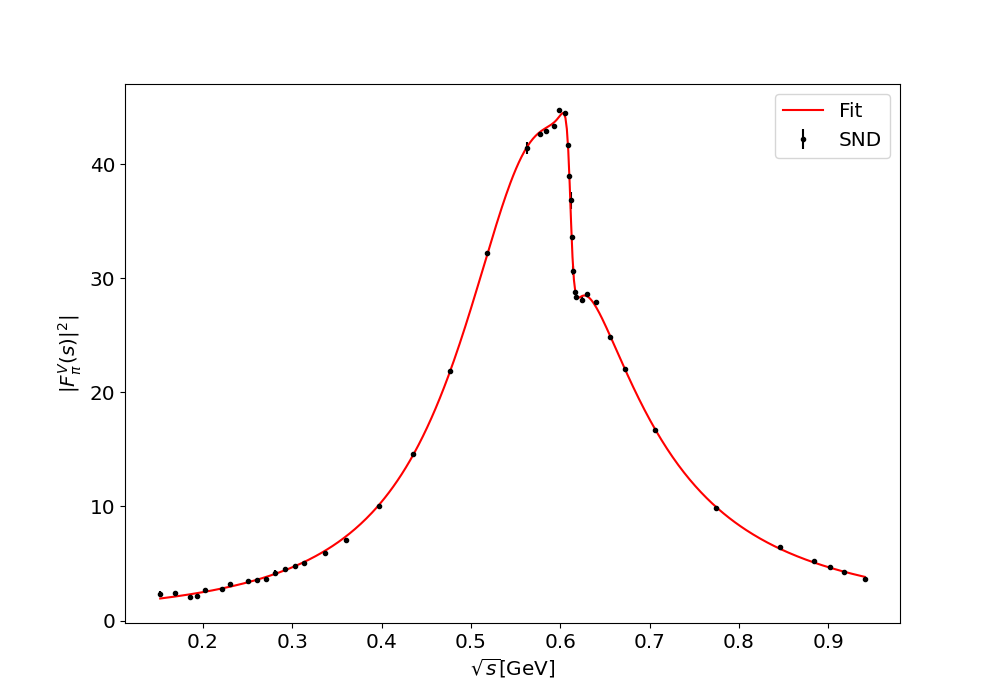
\includegraphics[width=0.8\textwidth]{./plots/SND.png}
    \caption{SND data fit\label{fig1}}
\end{figure}
\begin{figure}[H]
    \centering
    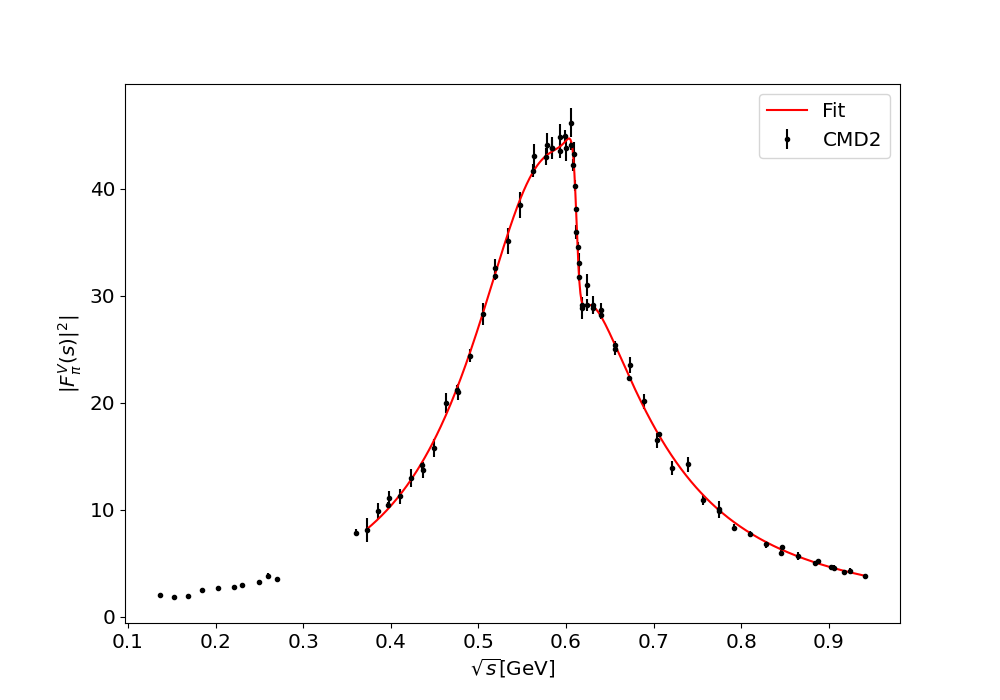
\includegraphics[width=0.8\textwidth]{./plots/CMD2.png}
    \caption{CMD2 data fit\label{fig2}}
\end{figure}
\begin{figure}[H]
    \centering
    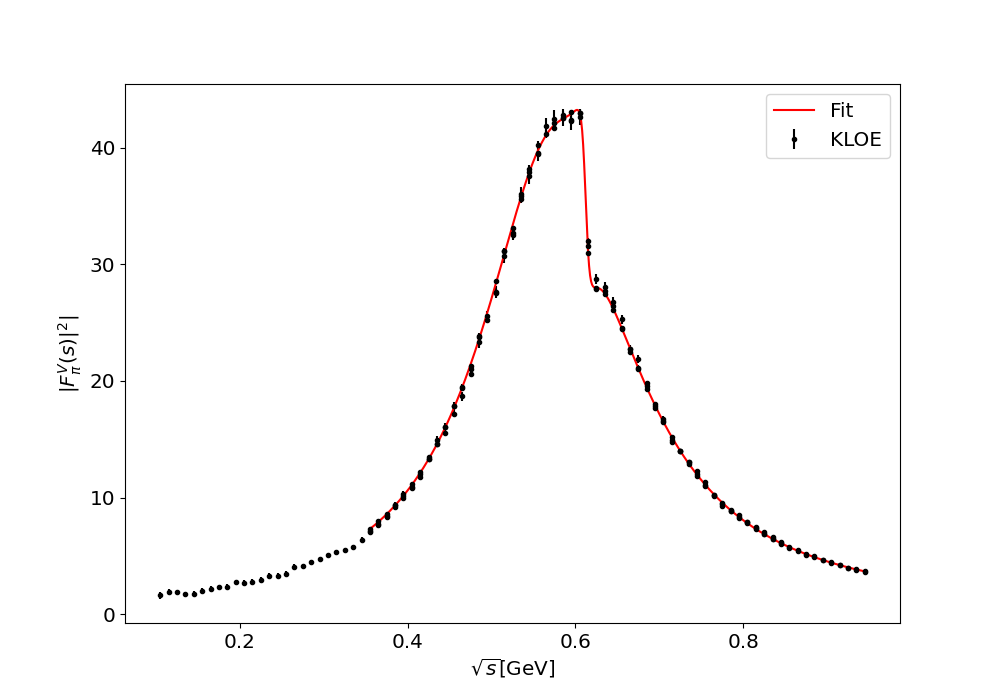
\includegraphics[width=0.8\textwidth]{./plots/KLOE.png}
    \caption{KLOE data fit\label{fig3}}
\end{figure}
\begin{figure}[H]
    \centering
    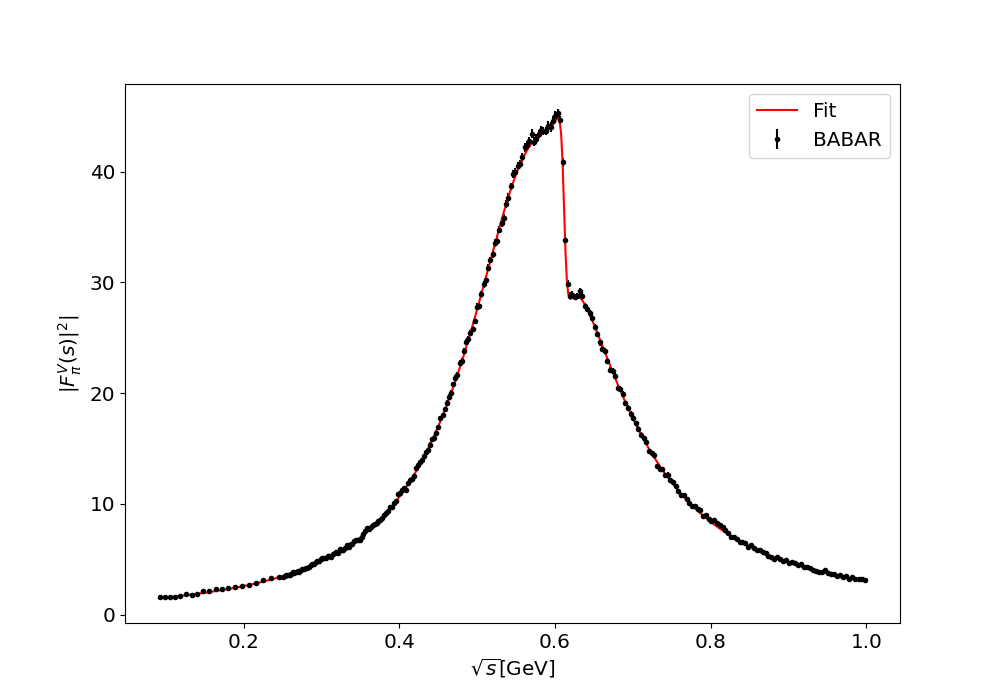
\includegraphics[width=0.8\textwidth]{./plots/BABAR.png}
    \caption{BABAR data fit\label{fig4}}
\end{figure}



\begin{figure}[H]
    \centering
    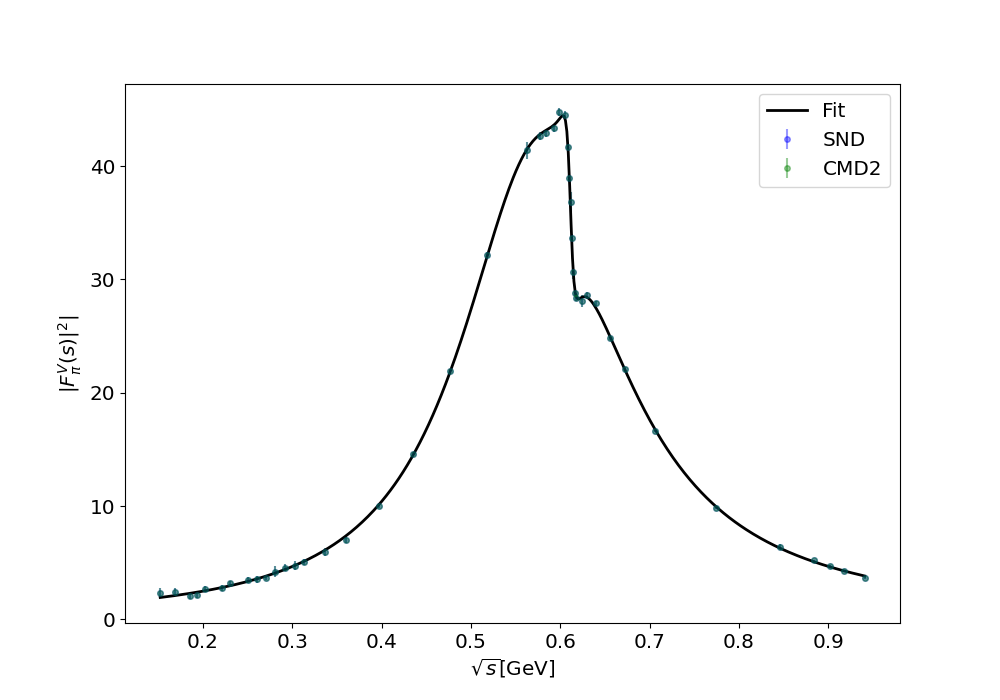
\includegraphics[width=0.8\textwidth]{./plots/SND-CMD2.png}
    \caption{SND and CMD2 fitted togther\label{fig5}}
\end{figure}
\begin{figure}[H]
    \centering
    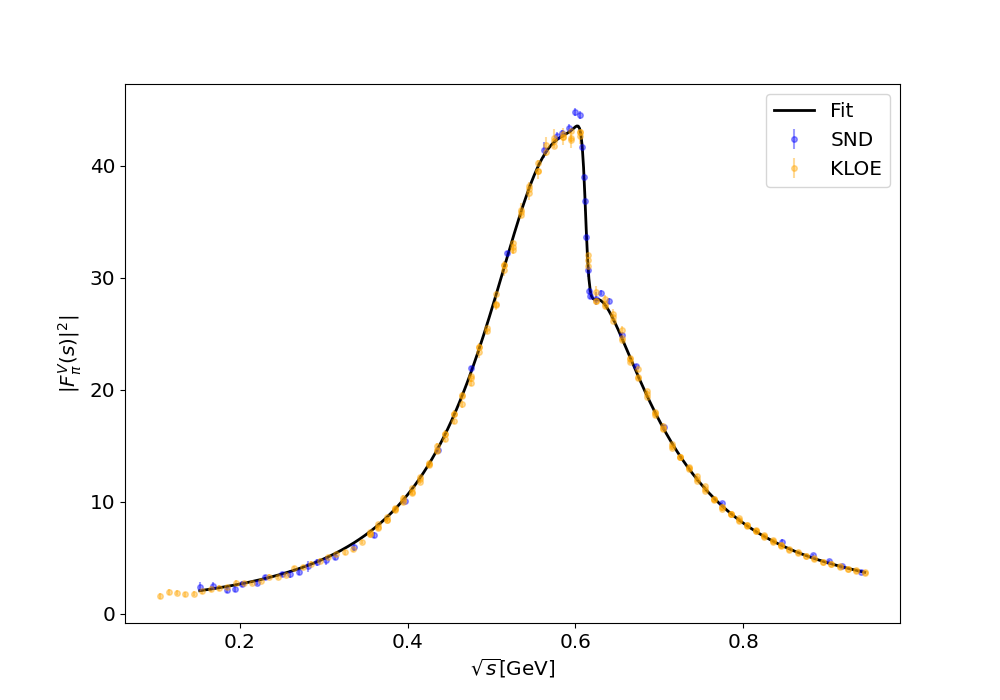
\includegraphics[width=0.8\textwidth]{./plots/SND-KLOE.png}
    \caption{SND and KLOE fitted togther    \label{fig6}}
\end{figure}
\begin{figure}[H]
    \centering
    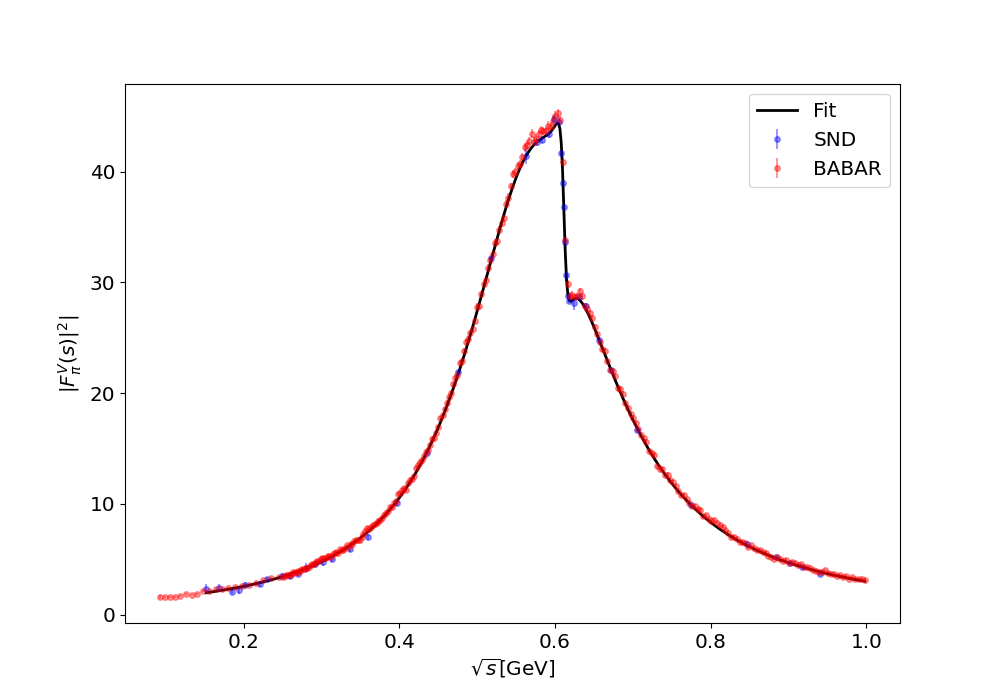
\includegraphics[width=0.8\textwidth]{./plots/SND-BABAR.png}
    \caption{SND and BABAR fitted togther   \label{fig7}}
\end{figure}


\begin{figure}[H]
    \centering
    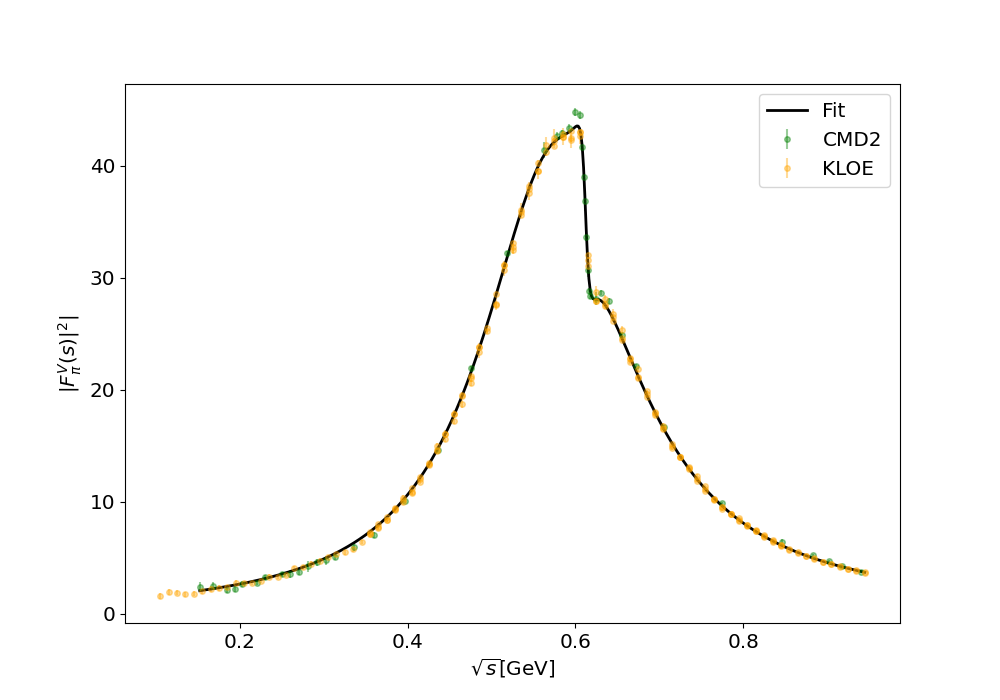
\includegraphics[width=0.8\textwidth]{./plots/CMD2-KLOE.png}
    \caption{CMD2 and KLOE fitted togther   \label{fig8}}
\end{figure}
\begin{figure}[H]
    \centering
    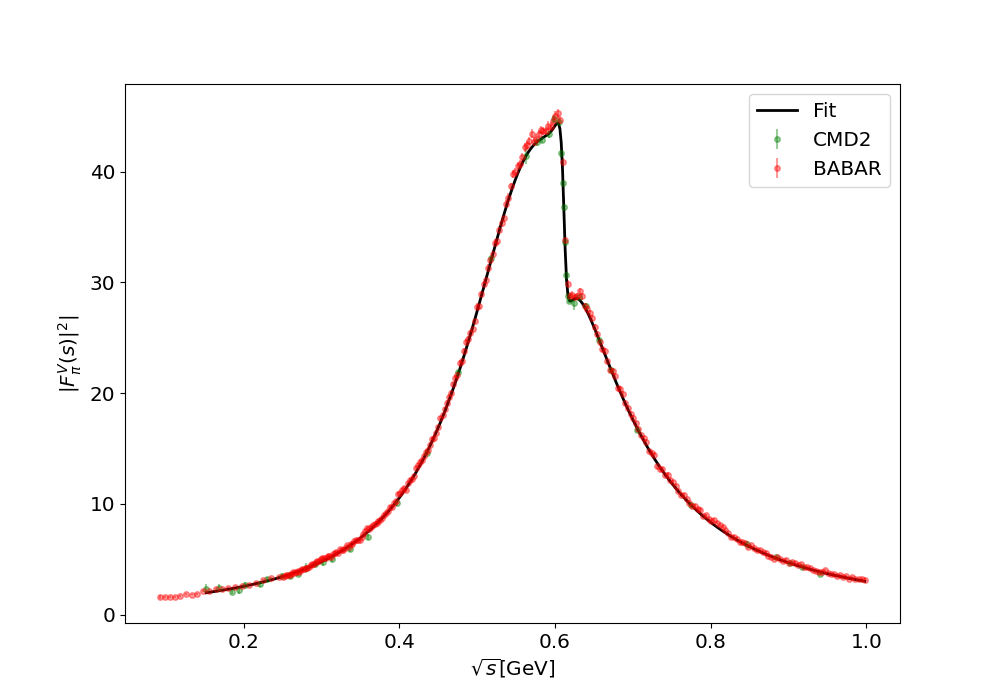
\includegraphics[width=0.8\textwidth]{./plots/CMD2-BABAR.png}
    \caption{CMD2 and BABAR fitted togther   \label{fig9}}
\end{figure}
\begin{figure}[H]
    \centering
    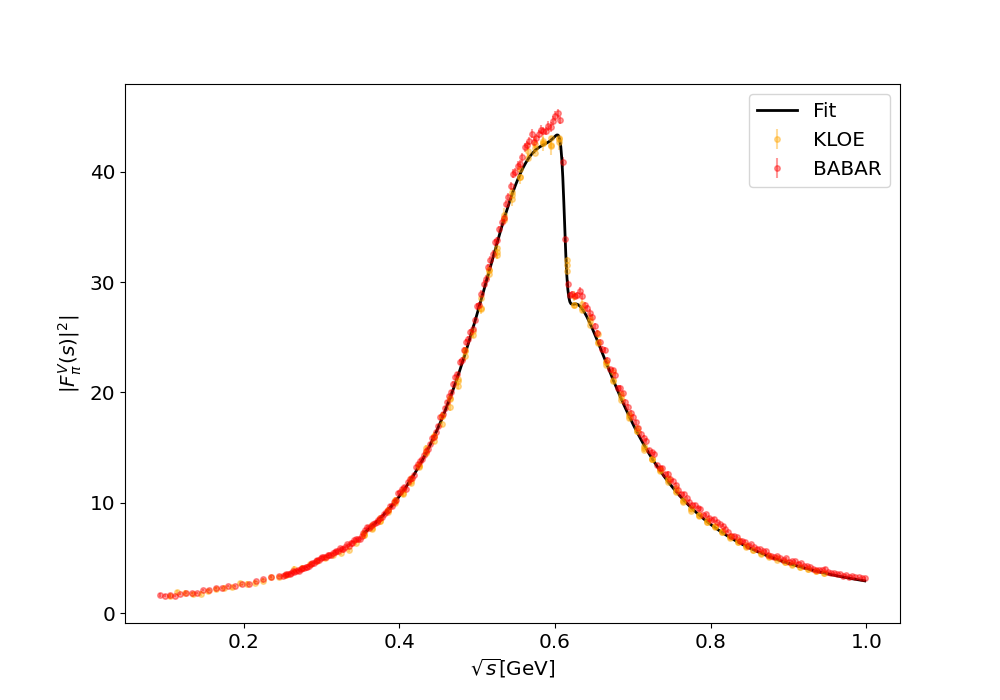
\includegraphics[width=0.8\textwidth]{./plots/KLOE-BABAR.png}
    \caption{KLOE and BABAR fitted togther   \label{fig10}}
\end{figure}

\begin{figure}[H]
    \centering
    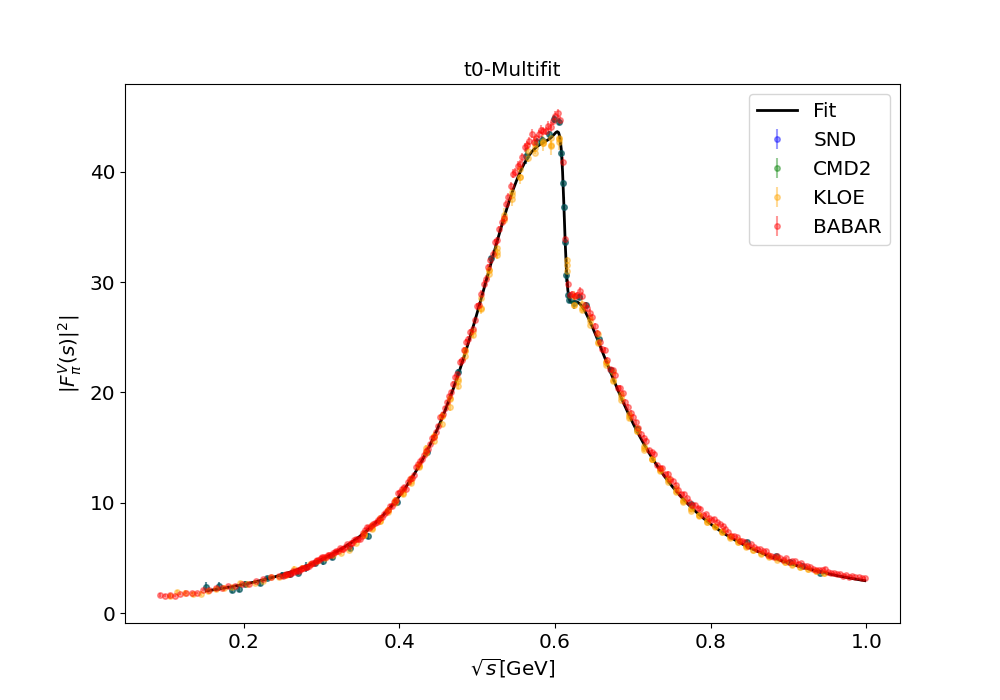
\includegraphics[width=0.8\textwidth]{./plots/multi.png}
    \caption{SND, CMD, KLOE and BABAR fitted togther   \label{fig11}}
\end{figure}

\begin{figure}[H]
    \centering
    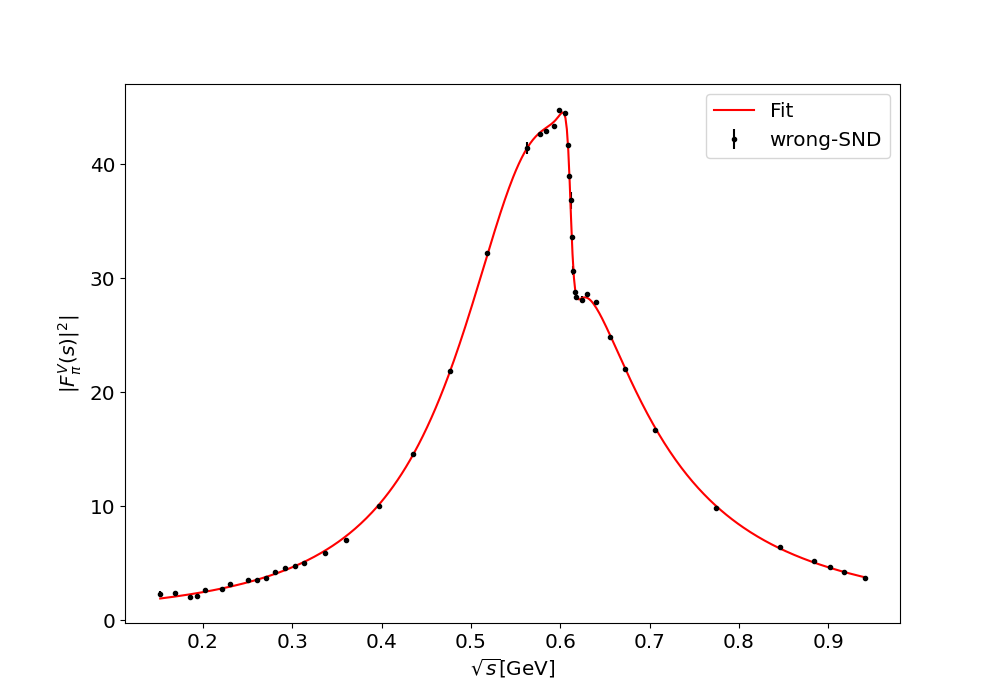
\includegraphics[width=0.8\textwidth]{./plots/wrong-SND.png}
    \caption{Wrong method, SND data fit\label{fig12}}
\end{figure}
\begin{figure}[H]
    \centering
    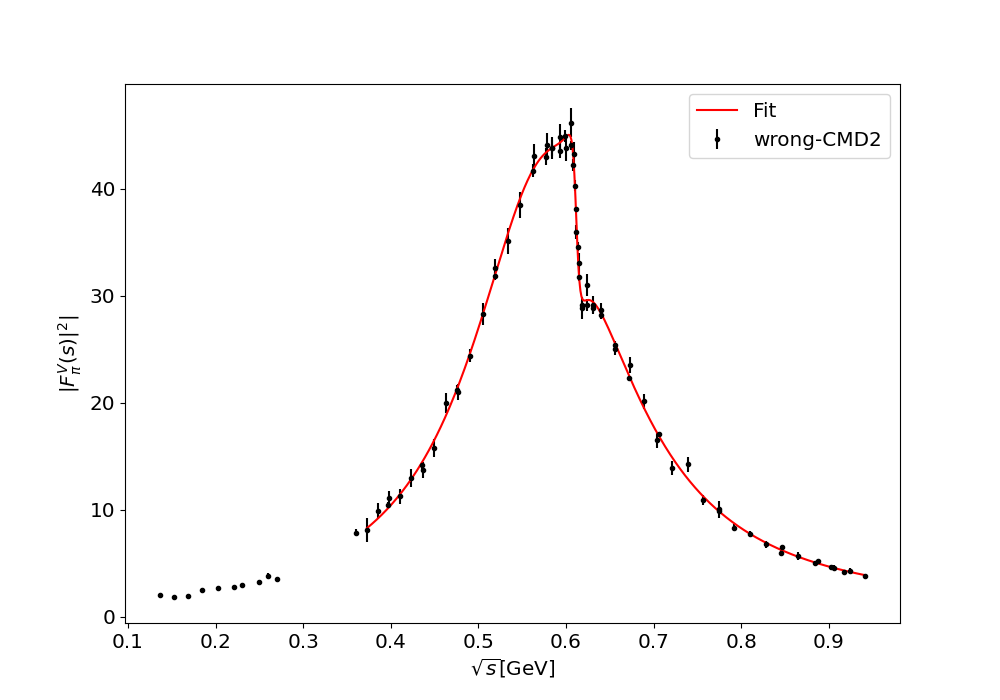
\includegraphics[width=0.8\textwidth]{./plots/wrong-CMD2.png}
    \caption{Wrong method, CMD2 data fit\label{fig13}}
\end{figure}
\begin{figure}[H]
    \centering
    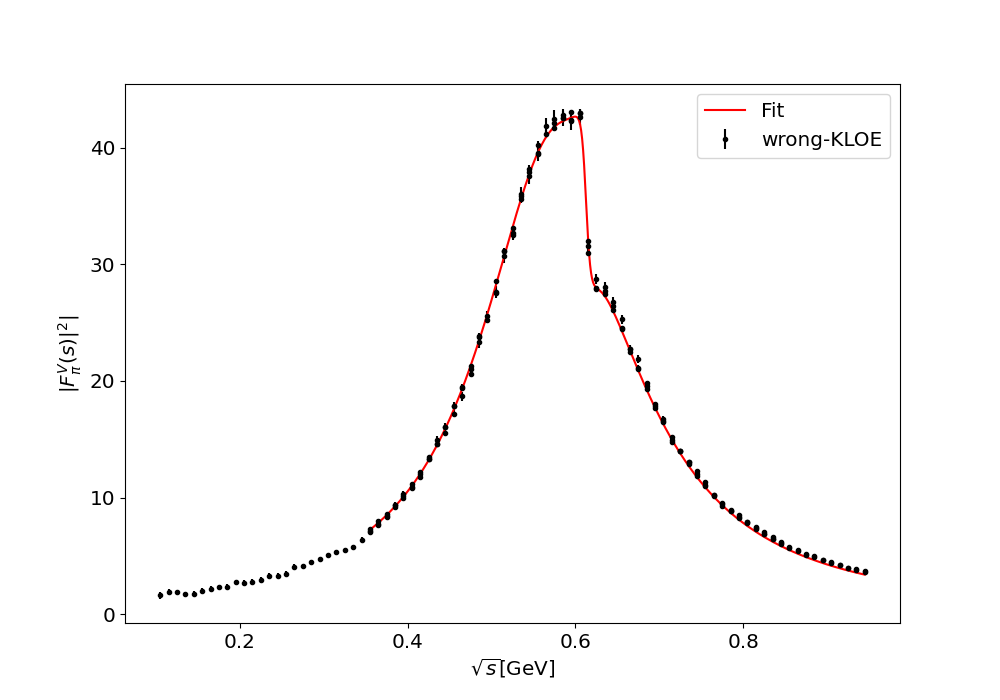
\includegraphics[width=0.8\textwidth]{./plots/wrong-KLOE.png}
    \caption{Wrong method, KLOE data fit\label{fig14}}
\end{figure}
\begin{figure}[H]
    \centering
    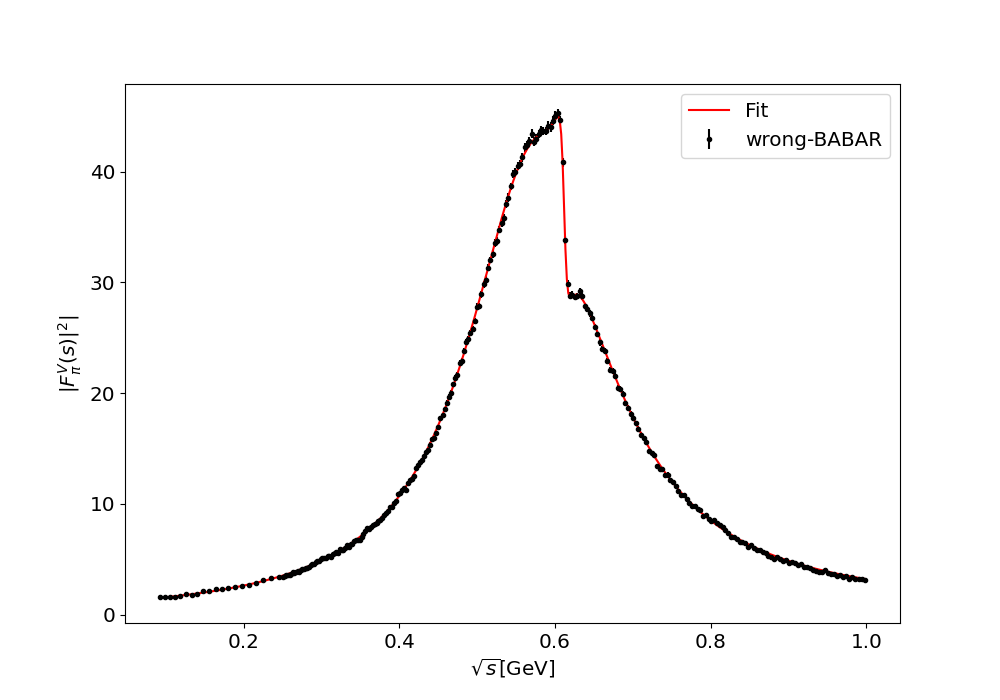
\includegraphics[width=0.8\textwidth]{./plots/wrong-BABAR.png}
    \caption{Wrong method, BABAR data fit\label{fig15}}
\end{figure}

\section{Conclusion}
Under consideration of the D'Agostini bias in the calculations we arrive very close the the literature values in table \ref{tabref}.
Furthermore the parameters in table \ref{tabsingle} all make the $\chi^2_{min}/dof$ value converge to $1$, making the goodnes of the fit very
good. When fitting two experiments together the results according to the $\chi^2_{min}/dof$ value are only good for SND-CMD2, SND-BABAR
and CMD2-BABAR, table \ref{tabtwo1} and \ref{tabtwo2}. Taking this into account we need to choose the experiments fitted together very
carefully to arrive at good results, fitting all experiments together for instance does't provide a good  $\chi^2_{min}/dof$ value, table
\ref{tabmulti}. Furthermore looking at the parameter fits without consideration of the D'Agostini bias we can conclude that the fits are
obviously missing something, table \ref{tabwrong}.

\printbibliography

\end{document}
